\documentclass[a4paper,14pt]{extreport}
	\usepackage[left=1.5cm,right=1.5cm,
	    top=1.5cm,bottom=2cm,bindingoffset=0cm]{geometry}
	\usepackage{scrextend}
	\usepackage[T1,T2A]{fontenc}
	\usepackage[utf8]{inputenc}
	\usepackage[english,russian,ukrainian]{babel}
	\usepackage{tabularx}
	\linespread{1.5}
	\usepackage{amssymb}
	\usepackage{fp}
	\usepackage{color}
	\usepackage{amsmath}
	\usepackage{mathrsfs}
	\usepackage{listings}
	\usepackage{graphicx}
	\graphicspath{ {./images/} }
	\usepackage{lipsum}
	\usepackage{xcolor}
	\usepackage{multirow}
	%\usepackage[table,xcdraw]{xcolor}
	\usepackage{hyperref}
	\usepackage{tcolorbox}
	\usepackage{tikz}
	\usepackage[framemethod=TikZ]{mdframed}
	\usepackage{wrapfig,boxedminipage,lipsum}
	\mdfdefinestyle{MyFrame}{%
	linecolor=blue,outerlinewidth=2pt,roundcorner=20pt,innertopmargin=\baselineskip,innerbottommargin=\baselineskip,innerrightmargin=20pt,innerleftmargin=20pt,backgroundcolor=gray!50!white}
	 \usepackage{csvsimple}
	 \usepackage{supertabular}
	\usepackage{pdflscape}
	\usepackage{fancyvrb}
	%\usepackage{comment}
	\definecolor{ggreen}{rgb}{0.4,1,0}
	\definecolor{rred}{rgb}{1,0.1,0.1}
	\definecolor{aquamarine}{rgb}{0.5, 1.0, 0.83}
	\definecolor{amber}{rgb}{1.0, 0.75, 0.0}
	\definecolor{babyblue}{rgb}{0.54, 0.81, 0.94}
	\definecolor{buff}{rgb}{0.94, 0.86, 0.51}
	\definecolor{internationalorange}{rgb}{1.0, 0.31, 0.0}
	\definecolor{lightmauve}{rgb}{0.86, 0.82, 1.0}
	\definecolor{mediumaquamarine}{rgb}{0.4, 0.8, 0.67}
	\usepackage{array,tabularx}
	\usepackage{colortbl}
	
	\usepackage{varwidth}
	\tcbuselibrary{skins}
	\usepackage{fancybox}

	\usetikzlibrary{calc}
	\makeatletter
	\newlength{\mylength}
	\xdef\CircleFactor{1.1}
	\setlength\mylength{\dimexpr\f@size pt}
	\newsavebox{\mybox}
	\newcommand*\circled[2][draw=blue]{\savebox\mybox{\vbox{\vphantom{WL1/}#1}}\setlength\mylength{\dimexpr\CircleFactor\dimexpr\ht\mybox+\dp\mybox\relax\relax}\tikzset{mystyle/.style={circle,#1,minimum height={\mylength}}}
	\tikz[baseline=(char.base)]
	\node[mystyle] (char) {#2};}
	\makeatother
	\usepackage{pgfplots}
    \pgfplotsset{compat=1.9}


	\usepackage{float}
	\usepackage{wrapfig}
	\usepackage{framed}
	%for nice Code{
	\lstdefinestyle{customc}{
	  belowcaptionskip=1\baselineskip,
	  breaklines=true,
	  frame=L,
	  xleftmargin=\parindent,
	  language=C,
	  showstringspaces=false,
	  basicstyle=\small\ttfamily,
	  keywordstyle=\bfseries\color{green!40!black},
	  commentstyle=\itshape\color{purple!40!black},
	  identifierstyle=\color{blue},
	  stringstyle=\color{orange},
	}
	\lstset{escapechar=@,style=customc}
	\usepackage{enumitem}

	% Цвета для гиперссылок
  \definecolor{linkcolor}{rgb}{1.0, 0.22, 0.0}% цвет ссылок
  \definecolor{urlcolor}{rgb}{0.4, 1.0, 0.0}% цвет гиперссылок
  \hypersetup{pdfstartview=FitH,  linkcolor=linkcolor,urlcolor=urlcolor,citecolor=red, colorlinks=true}
%}


\begin{document}
\newtcbox{\xmybox}[1][red]{on line, arc=7pt,colback=#1!10!white,colframe=#1!50!black, before upper={\rule[-3pt]{0pt}{10pt}},boxrule=1pt, boxsep=0pt,left=6pt,right=6pt,top=2pt,bottom=2pt}
\pagecolor{white}
\begin{titlepage}
	\begin{center}
	\large
	Національний технічний університет України \\ "Київський політехнічний інститут імені Ігоря Сікорського"


	Факультет Електроніки

	Кафедра мікроелектроніки
	\vfill

	\textsc{ЗВІТ}\\

	{\Large Про виконання лабораторної роботи №4\\
	з дисципліни: «Схемотехніка-2. Цифрова схемотехніка»\\[1cm]

	ТРИГЕРИ


	}
	\bigskip
	\end{center}
	\vfill

	\newlength{\ML}
	\settowidth{\ML}{«\underline{\hspace{0.4cm}}» \underline{\hspace{2cm}}}
	\hfill
	\begin{minipage}{1\textwidth}
	Виконавець:\\
	Студент 4-го курсу \hspace{4cm} $\underset{\text{(підпис)}}{\underline{\hspace{0.2\textwidth}}}$  \hspace{1cm}А.\,С.~Мнацаканов\\


	Перевірила: \hspace{5.9cm} $\underset{\text{(підпис)}}{\underline{\hspace{0.2\textwidth}}}$  \hspace{1cm}Г.\,С.~Порева\\

	\end{minipage}

	\vfill

	\begin{center}
	2021
	\end{center}
\end{titlepage}






\textbf{Мета роботи} - ознайомитися з принципом побудови і логікою роботи
тригерів на інтегральних логічних схемах, визначити основні параметри.

\begin{figure}[h]
	\center{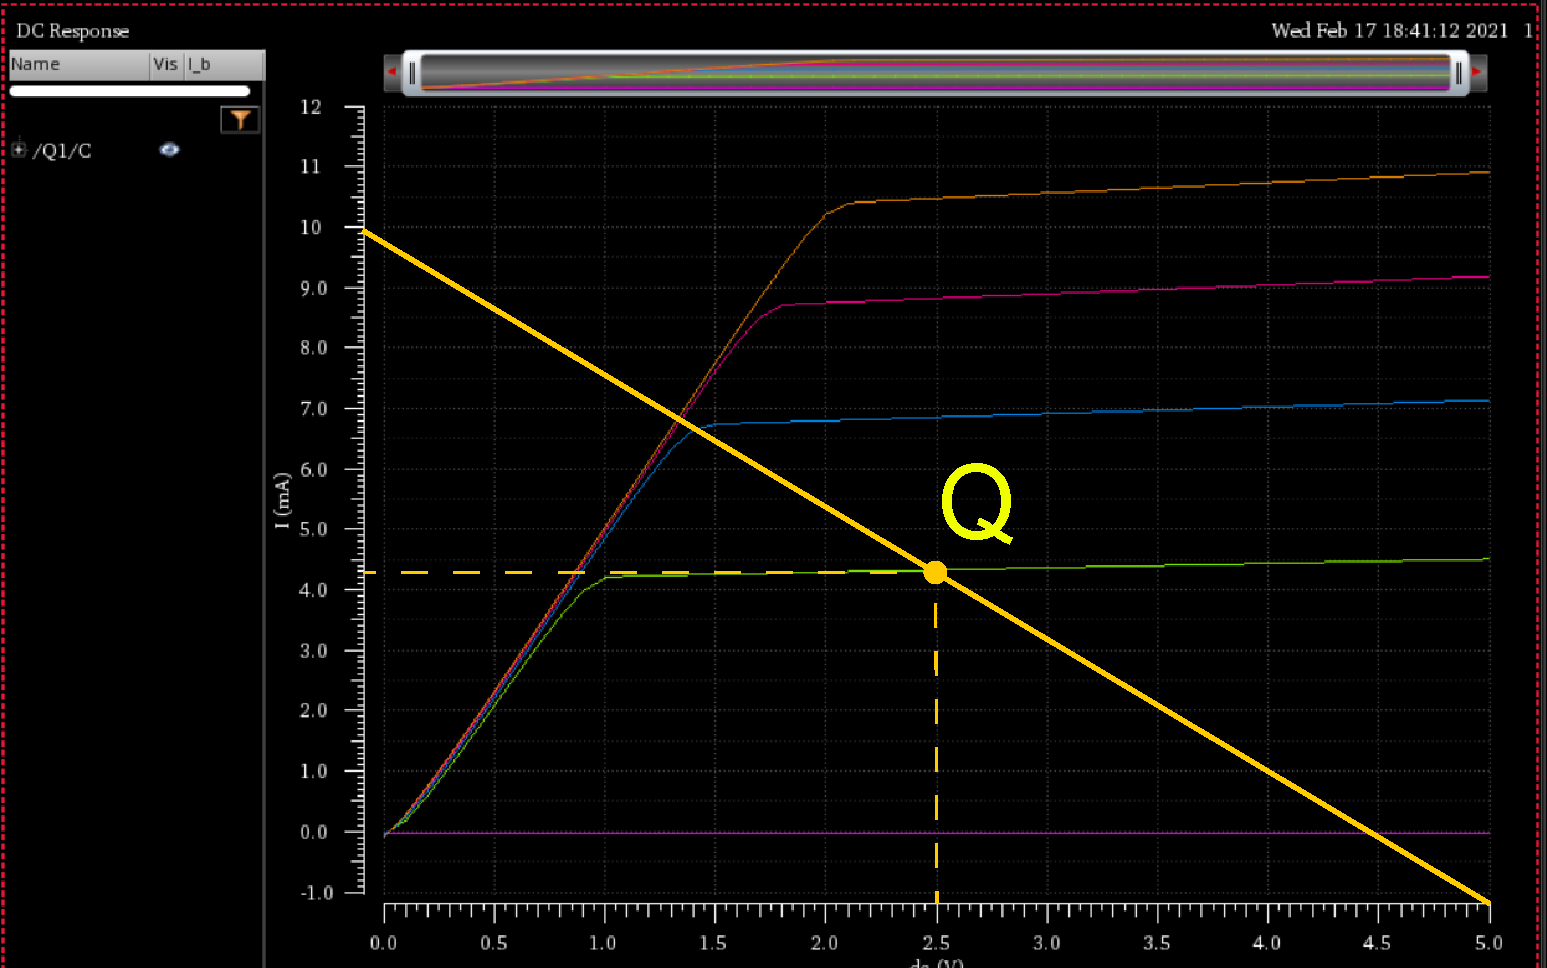
\includegraphics[width=0.7\linewidth]{1.png}}
	\caption{досліджувані схеми тригерів: RS-, S-, та D-тригери на логічних
елементах І-НІ.}
	\label{ris1}
\end{figure}


\begin{center}
\textbf{Робоче завдання}
\end{center}
Перемикачем лабораторних робіт, який знаходиться на задній панелі
стенда «ДИСКРЕТ М», включити роботу «ЛАБ 7».
Включити живлення стенду кнопкою «СЕТЬ».
Встановити на генераторі Г5-54 частоту проходження імпульсів f = 10
кГц. Основний імпульс (ОІ) позитивної полярності з амплітудою 5В,
тривалістю t і = 10мкс і затримкою t зт = 50 мкс щодо синхроімпульса (СІ) подати
на роз'єм «Ген. 1». Синхроімпульс позитивної полярності з амплітудою 5В
подати на роз'єм «Ген. 2». Використовувати зовнішню синхронізацію
осцилографа сигналом КТ15.

\begin{center}
\textbf{Виконання завдання}
\end{center}
 \begin{figure}[h!]
	\center{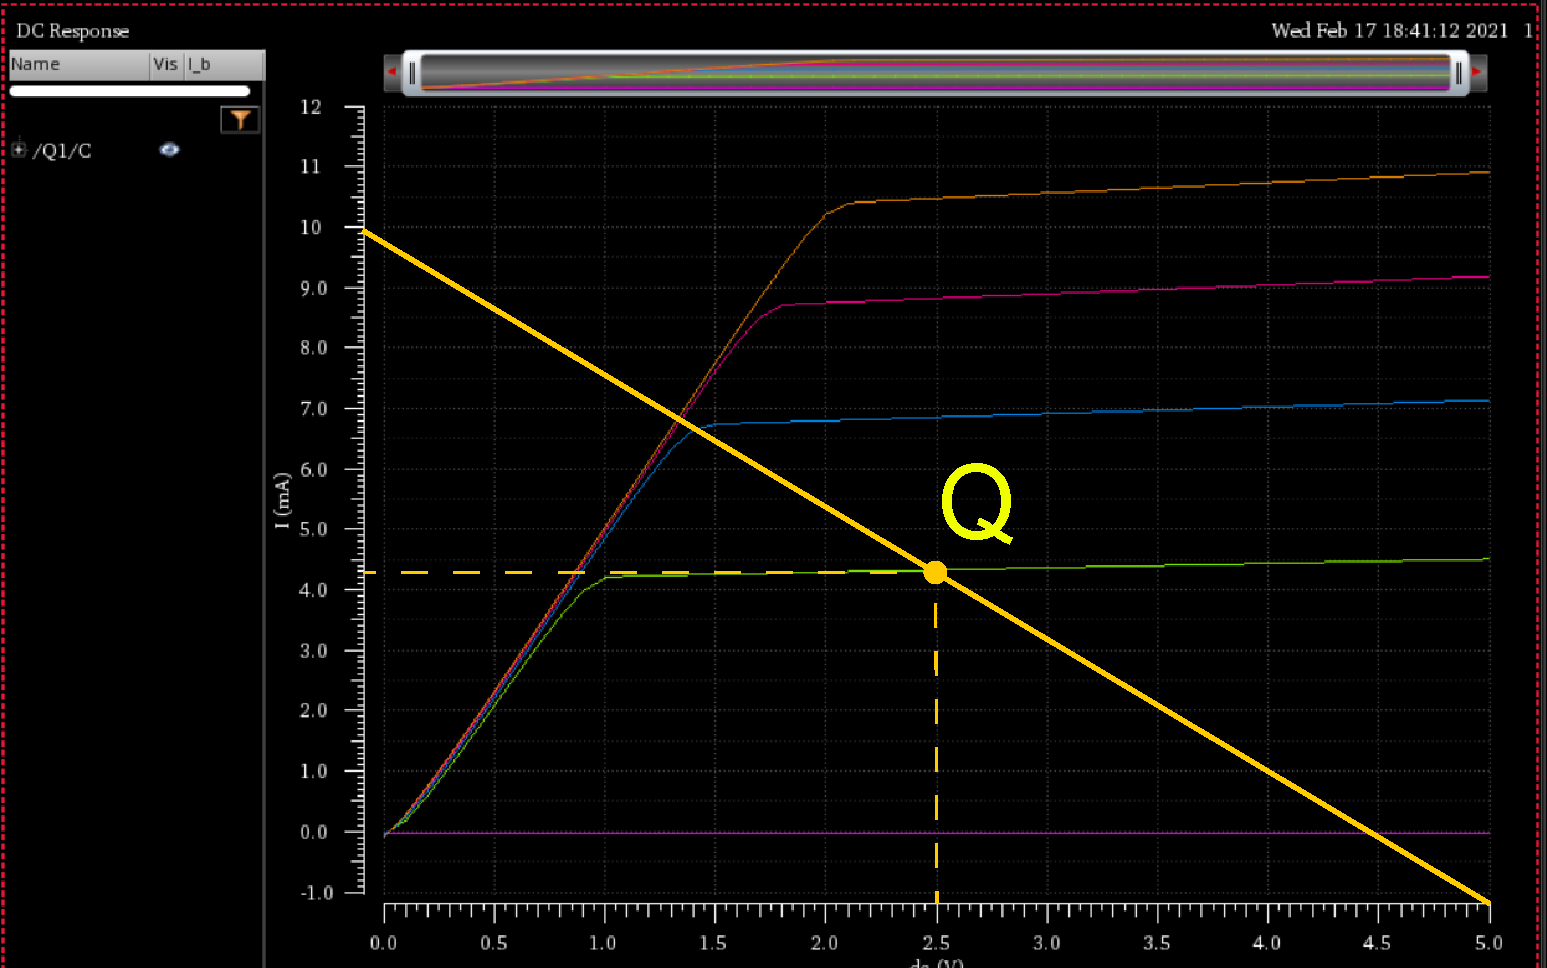
\includegraphics[width=0.8\linewidth, angle=-90]{1.jpg}}
	 \center{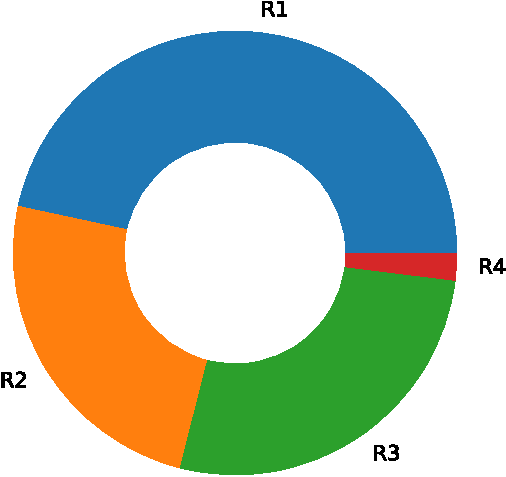
\includegraphics[width=0.8\linewidth]{2.jpg}}
	 
	  \end{figure}
 \begin{figure}[h!]
 
	 \center{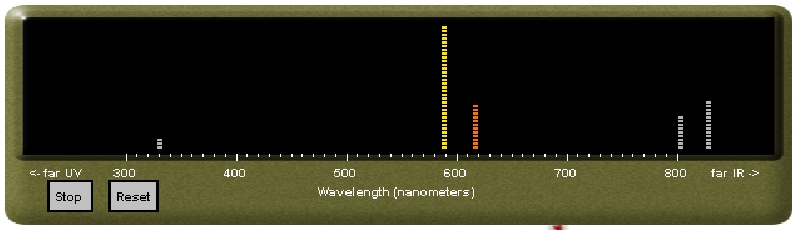
\includegraphics[width=0.8\linewidth]{3.jpg}}
	  \end{figure}
\clearpage 
\newpage
\begin{center}
\textbf{\fbox{Висновок}}
\end{center}

В роботі було досліджено роботу тригерів, як побудованих на окремих
елементах Шефера, так і вже готових. Виходячи з результатів саме JK-тригери є найкращим удосконаленням вiд за-
бороненої комбiнацiї.



 
 \begin{figure}[h!]
 
	 \center{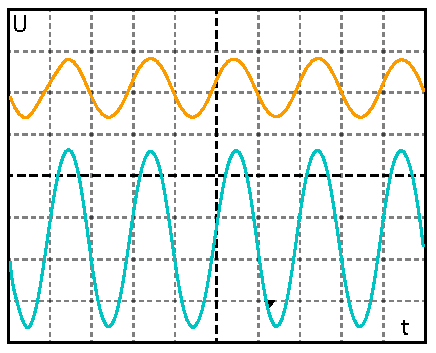
\includegraphics[width=0.8\linewidth]{4.jpg}}
	  \end{figure}





\end{document}